\documentclass{article}

% NeurIPS 2026 submission style. The default option is anonymous main-track
% review. Use [preprint] for arXiv drafts or [main, final] after acceptance.
\usepackage{neurips_2026}

\usepackage[utf8]{inputenc}
\usepackage[T1]{fontenc}
\usepackage{hyperref}
\usepackage{url}
\usepackage{booktabs}
\usepackage{amsfonts}
\usepackage{nicefrac}
\usepackage{microtype}
\usepackage{xcolor}
\usepackage{graphicx}
\usepackage{subfigure}
\usepackage{amsmath}
\usepackage{amssymb}
\usepackage{mathtools}
\usepackage{amsthm}
\usepackage[capitalize,noabbrev]{cleveref}

%%%%%%%%%%%%%%%%%%%%%%%%%%%%%%%%
% THEOREMS
%%%%%%%%%%%%%%%%%%%%%%%%%%%%%%%%
\theoremstyle{plain}
\newtheorem{theorem}{Theorem}[section]
\newtheorem{proposition}[theorem]{Proposition}
\newtheorem{lemma}[theorem]{Lemma}
\newtheorem{corollary}[theorem]{Corollary}
\theoremstyle{definition}
\newtheorem{definition}[theorem]{Definition}
\newtheorem{assumption}[theorem]{Assumption}
\theoremstyle{remark}
\newtheorem{remark}[theorem]{Remark}

\usepackage[disable,textsize=tiny]{todonotes}

\title{Brain States as Control Signals for Language Models: Mechanistic Evidence from TVB and Held-Out MEG}

\author{%
  Anonymous Author(s) \\
  Anonymous Institution \\
  \texttt{anonymous@example.com}
}

\begin{document}
\maketitle

\begin{abstract}
Language models are usually conditioned on text alone, yet many proposed continuous side signals can change output distributions without showing that the change is useful.
We study brain-state conditioning as a control problem and introduce a \emph{paired-control evaluation} principle: matched brain input should improve prediction over both removal controls (ZERO) and mismatch controls (SHUF), not merely deform the next-token distribution.
We quantify this distinction between generic perturbation and \emph{useful deformation} with Jensen-Shannon divergence (JSD) and next-token negative log-likelihood (NLL).
We intentionally evaluate this principle in two regimes.
In controlled synthetic TVB experiments, brain conditioning grows stronger with dimensionality, but only matched brain states improve NLL; shuffled and Gaussian-matched signals induce comparable deformation while harming prediction, and freezing the brain pathway removes all effects.
In real MEG-MASC, we use a T5 cross-attention model over post-word MEG windows and find that, after correcting decoder-context leakage and MEG scaling, matched MEG improves target-word NLL over both zeroed and shuffled MEG on random, story-blocked, and subject-blocked splits, with $\Delta$NLL gains of roughly $0.08$--$0.11$; leave-one-subject-out evaluation remains negative for all 11 held-out subjects.
The real effect is modest rather than full neural decoding, but it survives unseen-story evaluation and changes the top-1 prediction on about $10\%$ of held-out examples.
Together, these results argue that neural-state conditioning should be judged by paired controls and that this criterion reveals both strong synthetic mechanism and a modest but real held-out MEG alignment effect.
\end{abstract}

\section{Introduction}
\label{introduction}

Large language models (LMs) generate text by predicting the next token from preceding context, effectively treating language as a purely text-conditioned process.
Biological cognition, in contrast, is shaped by continuously evolving neural states reflecting perception, memory, affect, and internal dynamics.
This raises a natural modeling question: can a latent neural state serve as a \emph{control signal} that modulates linguistic prediction?

Prior work in brain-computer interfaces (BCI) has established that neural activity contains decodable information about intended communication, including handwriting and speech, using invasive recordings \citep{anumanchipalli2019speechsynthesis,makin2020handwriting,willett2021handwriting,moses2021neuroprosthesis,willett2023speechavatar}.
More recently, non-invasive recordings have been used to reconstruct aspects of continuous language semantics from fMRI \citep{tang2023semanticreconstruction}.
While these efforts primarily emphasize \emph{decoding} language from neural measurements, our focus is different: we treat a brain-state vector as an \emph{exogenous input} to a language model and ask whether it exerts measurable, structured control over the model's next-token distribution.

A second relevant thread is controllable generation.
Techniques such as attribute control and plug-and-play steering demonstrate that relatively low-dimensional signals can shift model behavior \citep{keskar2019ctrl,dathathri2020pplm}, and guidance methods in generative modeling formalize continuous ``control knobs'' for distribution shaping \citep{dhariwal2021diffusionbeatgans}.
However, output distributions can be substantially altered without improving next-token likelihood.
This motivates a mechanistic evaluation that separately measures (i) the magnitude of distributional deformation induced by control and (ii) whether this deformation increases probability mass on the correct continuation.

In this work, we study brain-conditioned language modeling under paired data of text contexts and multi-region brain-state vectors.
Rather than evaluating generation quality subjectively, we quantify brain influence by directly comparing next-token distributions with and without brain input.
For a context $x_{1:t}$ and brain state $z$, we measure deformation via Jensen-Shannon divergence between $p(\cdot\mid x_{1:t},z)$ and a zero-brain baseline $p(\cdot\mid x_{1:t},0)$, and we measure utility via next-token negative log-likelihood (NLL) on the ground-truth token.
This framework explicitly distinguishes generic perturbations from control signals that move probability mass toward correct predictions.
We apply this framework first to controlled synthetic TVB-derived signals, where we make our strongest mechanistic claims about dimensionality scaling, token sensitivity, and low-rank control geometry, and then to a real MEG-MASC pilot where the brain input is a temporal MEG window aligned to word onset.
For that real-neural regime, we denote the post-word MEG window by $B_{1:T}\in\mathbb{R}^{T\times C}$, where $T$ is the number of time bins and $C$ is the number of MEG sensors/channels.
Here TVB is used only as a whole-brain neurodynamical simulator that generates controlled synthetic neural trajectories.
It is not treated as a sentence-to-brain encoder and it does not provide real brain-language supervision; that role is reserved for MEG-MASC.
The real-data result is intentionally narrower: it asks whether any pairing-specific effect survives held-out evaluation, not whether the full synthetic picture transfers unchanged to real non-invasive recordings.
Our central claim is that neural-state conditioning should be judged by \emph{paired-control evaluation}: matched brain input must improve prediction over both removal and mismatch controls. Under this criterion, TVB reveals mechanism and held-out MEG reveals a modest but real alignment effect.


\begin{figure*}[t]
    \centering
    
\includegraphics[width=\linewidth]{pipeline.png}
    \caption{
    Brain-conditioned language modeling as controllable next-token distribution deformation.
    A brain snapshot $z$ is encoded into a control vector $a$ and injected into a Transformer LM's hidden states.
    We compare the resulting next-token distribution $p(\cdot\mid x,z)$ against the zero-brain baseline $p(\cdot\mid x,0)$ using Jensen-Shannon divergence (JSD), top-1 agreement, and $\Delta$NLL.
    }
    \label{fig:pipeline}
\end{figure*}


\paragraph{Contributions.}
(i) We introduce \emph{paired-control evaluation} for neural-state conditioning: brain input should be judged by whether it produces \emph{useful deformation}, improving prediction over both ZERO and SHUF controls rather than merely changing the output distribution.
(ii) In synthetic TVB experiments, we use this criterion to identify mechanism: control strength scales with dimensionality, deformation concentrates more strongly on content-bearing tokens, and both helpful and harmful signals act through a compact low-dimensional control subspace.
(iii) On real MEG-MASC recordings, we show that the same criterion survives held-out evaluation: a T5 cross-attention model with post-word MEG windows improves target-word NLL over both ZERO and SHUF on random, story-blocked, and subject-blocked splits after correcting decoder leakage and signal-scale failures, and remains negative for every held-out subject in leave-one-subject-out evaluation.
(iv) We provide diagnostic analyses and negative results that sharpen the claim rather than soften it, including frozen-pathway controls, failed peri-word and leakage-prone setups, and attention analyses showing that pairing-specific gains are more visible in NLL than in coarse attention timing.





\section{Brain-Conditioned Language Modeling and Evaluation}

Let $x_{1:t}$ denote a sequence of tokens and $z \in \mathbb{R}^d$ a brain-state vector representing activity across $d$ regions.
We train an autoregressive language model parameterized by $\theta$ to predict the next token conditioned on both text and brain state:
\begin{equation}
p_\theta(x_{t+1} \mid x_{1:t}, z) = \mathrm{softmax}\!\left(f_\theta(x_{1:t}, z)\right).
\end{equation}

The model is trained using standard next-token cross-entropy:
\begin{equation}
\mathcal{L}(\theta) = - \sum_{t} \log p_\theta(x_{t+1} \mid x_{1:t}, z).
\end{equation}

Brain conditioning is implemented via a learned projection that injects $z$ into the transformer hidden states.
When $z=\mathbf{0}$, the model reduces to a standard text-only LM.

For the real MEG-MASC pilot, the brain input is temporal rather than a single snapshot.
We use a post-word MEG window $B_{1:T}\in\mathbb{R}^{T\times C}$, project it with a small temporal brain encoder, and feed the resulting sequence to a T5 encoder-decoder model via encoder-side continuous embeddings.
The T5 decoder predicts target word tokens while cross-attending to the encoded MEG sequence.
This architecture preserves temporal structure and lets us evaluate whether the correct MEG window improves prediction over zeroed or shuffled brain controls.






\subsection{Paired-Control Evaluation of Brain Influence}


For a fixed context $x_{1:t}$, we compare:
\begin{align}
p &= p_\theta(\cdot \mid x_{1:t}, z), \\
q &= p_\theta(\cdot \mid x_{1:t}, \mathbf{0}).
\end{align}

We measure their divergence using Jensen-Shannon divergence:
\begin{equation}
\mathrm{JSD}(p \parallel q) = \frac{1}{2}\mathrm{KL}(p \parallel m) + \frac{1}{2}\mathrm{KL}(q \parallel m),
\quad m = \tfrac{1}{2}(p+q).
\end{equation}

We additionally report top-1 agreement, the fraction of samples for which $\arg\max p = \arg\max q$.
Together, these metrics quantify both how strongly the brain state alters token-level predictions and whether that deformation is useful under paired controls.




\subsection{Data}

We construct paired datasets of $(x_{1:t}, z, x_{t+1})$ triples by combining text from a fixed general-domain corpus derived from Wikipedia (Wiki-40B; following \cite{raffel2020t5}) with simulated multi-region brain activity generated using The Virtual Brain (TVB) \cite{schirner2022brain}.
TVB is a whole-brain dynamical simulator, not a language-to-brain model.
In this paper, we use it only to generate controlled synthetic neural trajectories for scaling, ablation, and perturbation experiments under known conditions.
It therefore supports mechanistic analysis of brain-conditioned control, while all claims about real brain-language alignment are evaluated on MEG-MASC rather than inferred from TVB.
We extract brain snapshots $z \in \mathbb{R}^d$ from $d$ cortical regions at matched time points.
We build separate datasets for brain dimensionalities
\[
d \in \{68, 136, 272, 544\},
\]
each containing approximately 100k samples.
For each $d$, a separate LM is trained to ensure architectural compatibility.

For real-neural validation, we use MEG-MASC \citep{gwilliams2023megmasc}, a natural-speech MEG dataset with word- and phoneme-level timing annotations.
We preprocess KIT MEG recordings, build word-aligned examples, and use post-word windows from $0.0$ to $0.6$ seconds after word onset.
The real-data pilot contains 200k word-aligned examples.
To avoid text leakage, the decoder is trained in a target-only mode: it receives shifted target tokens, but not the preceding story context.
The brain window is normalized per example before the temporal brain encoder.
We report random train/test splits, story-blocked held-out evaluation to reduce story-level leakage, subject-blocked evaluation, and leave-one-subject-out (LOSO) subject generalization.

\section{Experiments}
\label{sec:experiments}

The experiments are split into two regimes.
Sections~\ref{sec:dim}--\ref{sec:scaling} study controlled synthetic TVB-derived signals to establish mechanism under known conditions, while Section~\ref{sec:megmasc_pilot} uses real MEG-MASC recordings to test whether the same REAL/ZERO/SHUF logic survives held-out evaluation on measured neural data.


\begin{table*}[t]
\centering
\caption{Brain influence increases with brain dimensionality. JSD is computed between next-token distributions with real brain input vs.\ zeroed brain.}
\label{tab:js_results}
\begin{tabular}{lcccc}
\toprule
Brain dim & JSD mean & JSD median & JSD std & Top-1 agree \\
\midrule
68  & 0.0657 & 0.0511 & 0.0604 & 0.681 \\
136 & 0.0736 & 0.0540 & 0.0696 & 0.660 \\
272 & 0.0857 & 0.0718 & 0.0710 & 0.620 \\
544 & 0.1359 & 0.1162 & 0.1073 & 0.577 \\
\bottomrule
\end{tabular}
\end{table*}




\begin{table*}
\centering
\caption{Controls for the 136-D brain-conditioned model.
Real brain conditioning improves next-token likelihood despite inducing distributional deformation comparable to shuffled and Gaussian controls.}
\label{tab:controls-136}
\begin{tabular}{lcccc}
\toprule
Condition & JS mean & Top-1 agree & NLL mean & $\Delta$NLL vs.\ ZERO \\
\midrule
REAL  & 0.0737 & 0.661 & 2.417 & $-0.376$ \\
ZERO  & -    & 1.000 & 2.793 & 0.000 \\
SHUF  & 0.0756 & 0.655 & 2.931 & $+0.138$ \\
GAUSS & 0.0739 & 0.654 & 2.932 & $+0.139$ \\
\bottomrule
\end{tabular}
\end{table*}

We evaluate whether brain snapshots act as a structured control input for next-token prediction, and whether observed distribution shifts reflect meaningful brain-text alignment rather than generic perturbation. Unless noted otherwise, all metrics are computed on 5{,}000 held-out contexts.

\subsection{Synthetic TVB: control strength scaling with brain dimensionality}
\label{sec:dim}

We test whether higher-dimensional brain snapshots yield stronger modulation of the model's next-token distribution.
For each $d \in \{68,136,272,544\}$, we train a brain-conditioned LM using the same text corpus, architecture family, and optimization settings, varying only the brain snapshot dimensionality $z \in \mathbb{R}^d$ and the corresponding brain-to-hidden projection.

To quantify control strength, we measure how much the next-token distribution changes when conditioning on a real brain snapshot, relative to a zero-brain baseline.
Concretely, for each $d$ we compute Jensen-Shannon divergence (JSD) between $p(\cdot \mid x_{1:t}, z)$ and $p(\cdot \mid x_{1:t}, \mathbf{0})$, along with top-1 agreement as a measure of argmax stability.

Table~\ref{tab:js_results} summarizes these metrics across dimensionalities. Mean JSD increases monotonically with $d$ ($0.066 \rightarrow 0.136$), while top-1 agreement decreases ($0.681 \rightarrow 0.577$), indicating that richer brain representations produce larger and more frequent shifts in token probabilities relative to the text-only baseline.




\subsection{Synthetic TVB: separating generic perturbation from aligned signal}
\label{sec:controls}

A central challenge in evaluating external control signals is that distributional change alone is not informative.
Injecting almost any additional vector into a language model can deform logits, alter the argmax token, and increase divergence from a baseline-without improving prediction.
To claim that brain snapshots provide meaningful control, we must therefore show that their effects cannot be replicated by unstructured or misaligned perturbations.



\paragraph{Control conditions.}
For each evaluation context, we consider four conditioning regimes:
(i) \textbf{REAL}, the true brain vector paired with the text;
(ii) \textbf{ZERO}, an all-zero brain vector;
(iii) \textbf{SHUF}, brain vectors randomly permuted across samples, preserving marginal statistics but breaking alignment;
(iv) \textbf{GAUSS}, Gaussian vectors matched to the empirical mean and variance of the brain dataset.

For each condition, we compare the resulting next-token distribution to the ZERO baseline.
We report (a) Jensen-Shannon divergence (JSD) as a measure of distributional deformation,
(b) top-1 agreement as a measure of argmax stability, and
(c) next-token negative log-likelihood (NLL) on the ground-truth token.
Changes in predictive performance are summarized as $\Delta$NLL relative to ZERO.

Table~\ref{tab:controls-136} reveals a clear dissociation between deformation magnitude and predictive usefulness.
All non-zero conditioning vectors-REAL, SHUF, and GAUSS-induce comparable Jensen-Shannon divergence relative to ZERO, confirming that substantial distributional deformation is easy to obtain.
Likewise, all three reduce top-1 agreement to a similar extent, indicating frequent changes to the argmax token.

Crucially, only the REAL brain condition improves next-token prediction.
Conditioning on the true brain vector reduces NLL by $0.376$, while both SHUF and GAUSS \emph{worsen} prediction despite inducing nearly identical distributional shifts.
This demonstrates that the benefit of brain conditioning cannot be attributed to generic perturbation, added variance, or increased expressivity alone.
Instead, predictive gains depend on structured alignment between the brain state and the linguistic context.

\paragraph{Frozen pathway control.}
To verify that these effects are mediated by the learned brain-conditioning mechanism itself, we perform an additional causal control by freezing the brain projection to zero.
Under this intervention, all conditioning regimes collapse to the ZERO baseline: Jensen-Shannon divergence drops to zero, top-1 agreement returns to one, and NLL becomes identical across REAL, SHUF, and GAUSS.
This confirms that both distributional deformation and predictive gains arise specifically from the learned brain injection pathway, rather than from incidental architectural or evaluation artifacts.

\subsection{Real MEG-MASC pilot: held-out alignment under blocked splits}
\label{sec:megmasc_pilot}

We next test whether the same REAL/ZERO/SHUF logic transfers to real neural recordings.
Using MEG-MASC, we train a T5 encoder-decoder model in which a temporal brain encoder maps a post-word MEG window ($0.0$--$0.6$ seconds after word onset) into T5 encoder embeddings, and the decoder predicts the target word tokens via cross-attention.
The final model is trained with target-only decoder inputs to reduce leakage from text context, per-example brain normalization, and a mostly frozen T5 in which we unfreeze decoder cross-attention in the last six blocks together with the final decoder block.

This pilot exposed two important negative results before producing a usable signal.
First, when decoder-side text context was available under standard teacher forcing, REAL, ZERO, and SHUF controls were essentially indistinguishable: the language model could rely on text priors without using MEG.
Second, an initial z-scoring implementation added a fixed $10^{-6}$ constant to channel standard deviations.
Because raw MEG values are stored in very small physical units, this collapsed the effective brain inputs toward zero; a diagnostic batch had mean absolute input magnitude $\approx 1.4\times 10^{-7}$ and nearly identical logits for REAL and ZERO.
After correcting these issues, a conservative cross-attention-only model produced only a tiny in-sample effect (reported in Appendix~\ref{app:meg_t5_diagnostics}).
We therefore evaluate the stronger post-word hybrid configuration on three held-out regimes: a standard random split, a story-blocked split that withholds entire stories at test time, and a subject-blocked split. We then test subject generalization more aggressively with leave-one-subject-out (LOSO) evaluation over all 11 subjects.

\begin{table*}[t]
\centering
\caption{Held-out MEG-MASC/T5 results for the post-word hybrid model (target-only decoding, per-example brain normalization). REAL uses the matched MEG window, ZERO removes the MEG input, and SHUF permutes MEG windows across examples. Negative $\Delta$NLL means REAL is better.}
\label{tab:megmasc_t5}
\resizebox{\linewidth}{!}{%
\begin{tabular}{lccccccccc}
\toprule
Split & $n$ & NLL REAL & NLL ZERO & NLL SHUF & $\Delta$R-Z & 95\% CI & $\Delta$R-S & 95\% CI & Top-1 R/Z \\
\midrule
Random held-out & 17{,}976 & 5.9661 & 6.0719 & 6.0817 & $-0.1057$ & [$-0.1141$, $-0.0974$] & $-0.1155$ & [$-0.1232$, $-0.1079$] & 0.8745 \\
Story-blocked & 50{,}000 & 7.1885 & 7.2933 & 7.2663 & $-0.1048$ & [$-0.1092$, $-0.1004$] & $-0.0778$ & [$-0.0818$, $-0.0738$] & 0.8997 \\
Subject-blocked & 34{,}240 & 5.9947 & 6.0742 & 6.0771 & $-0.0795$ & [$-0.0845$, $-0.0744$] & $-0.0824$ & [$-0.0871$, $-0.0776$] & 0.9954 \\
\bottomrule
\end{tabular}
}
\end{table*}

Table~\ref{tab:megmasc_t5} shows that real MEG improves NLL over both zeroed and shuffled MEG on both held-out splits.
On the random split, REAL beats ZERO by $0.1057$ NLL and SHUF by $0.1155$, with both paired confidence intervals fully below zero.
More importantly, the effect survives the stricter story-blocked evaluation: REAL remains better than ZERO by $0.1048$ NLL and better than SHUF by $0.0778$.
The same pattern persists under subject-blocked evaluation, where REAL still beats ZERO by $0.0795$ NLL and SHUF by $0.0824$ on unseen subjects.
This makes the result substantially stronger than the earlier tiny in-sample cross-attention-only pilot.
At the same time, it is still not open-vocabulary word decoding.
Top-1 agreement with the ZERO baseline remains around $0.87$--$0.90$, so the correct MEG window changes the preferred token for only a minority of examples.
We therefore interpret the result as modest but genuine held-out neural alignment: the matched MEG signal shifts probability mass toward the target more than either no brain input or mismatched brain input, and it does so even on unseen stories.
To make the effect size more concrete, a $\Delta$NLL of $-0.1048$ corresponds to an approximately $e^{0.1048}\!\approx\!1.11\times$ multiplicative increase in target-token probability under REAL relative to ZERO, while the story-blocked REAL-vs.\ SHUF gap of $-0.0778$ corresponds to about $e^{0.0778}\!\approx\!1.08\times$.
LOSO evaluation strengthens this further: for every held-out subject, both REAL-ZERO and REAL-SHUF remain negative, with mean subject-level effects of $-0.0819 \pm 0.0189$ and $-0.0796 \pm 0.0233$ (mean $\pm$ s.d. across 11 subjects), and all 22 subject-level 95\% confidence intervals below zero.
As a null auxiliary baseline, we also replace each MEG window with a matched-shape Gaussian control stream and retrain the same story-blocked architecture.
This auxiliary stream fails to produce a pairing-specific gain: REAL and SHUF become indistinguishable ($\Delta$R-S $\approx 0.00001$, 95\% CI spanning zero), with negligible deformation (JSD $\approx 6\times10^{-5}$, top-1 agreement with ZERO $\approx 0.999$).
A temporal ablation on the story-blocked split sharpens this interpretation.
Restricting the model to the early post-word half ($0.0$--$0.3$ s) collapses the effect ($\Delta$R-Z $\approx -7\times10^{-5}$, $\Delta$R-S $\approx 0$), while the late half ($0.3$--$0.6$ s) retains only a weaker signal ($-0.0227$, $-0.0206$).
A narrower late slice ($0.45$--$0.6$ s) fails entirely ($\Delta$R-Z $= +0.0005$, $\Delta$R-S $\approx 0$).
Thus, the useful MEG signal is post-word but distributed across the broader $0.0$--$0.6$ s response rather than concentrated in a single late peak.
This is meaningful as a held-out token-level effect, but it is still far from the regime where MEG alone would drive fluent sequence generation or robust word decoding.

\subsection{Synthetic TVB: dose-response scaling of the brain signal}
\label{sec:scaling}

To test whether brain conditioning behaves like a graded control knob, we scale the brain vector $z \leftarrow \alpha z$ with $\alpha \in \{0,0.25,0.5,1,2\}$.
For each $\alpha$, we report JSD and $\Delta$NLL relative to $\alpha=0$.

For both REAL and SHUF, JSD typically increases with $\alpha$, indicating smooth growth in deformation magnitude.
However, REAL and SHUF differ in predictive effect: REAL tends to reduce NLL for moderate $\alpha$, while SHUF degrades NLL despite comparable deformation.
The detailed alpha-scaling plots are moved to Appendix~\ref{app:alpha_scaling} to keep the main text focused on the control logic and real-MEG result.

\subsection{Token-level sensitivity: semantic vs.\ syntactic control}

To assess whether brain conditioning preferentially modulates semantic content rather than surface-level structure, we perform a lightweight token sensitivity analysis.
For each evaluation context, we compute the absolute logit change induced by brain conditioning,
\[
|\Delta \ell| = \left| \ell(x \mid z) - \ell(x \mid 0) \right|,
\]
and group vocabulary items into three coarse linguistic categories:
(i) punctuation, (ii) stopwords (function words), and (iii) content tokens (nouns, verbs, adjectives, numerals).

Table~\ref{tab:token_sensitivity_controls} reports mean $|\Delta \ell|$ for each token category under real, shuffled, and Gaussian brain inputs in the 136-D model.
Across all conditions, content tokens exhibit consistently larger logit changes than stopwords (content/stopword ratio $\approx 1.11\times$), indicating that brain conditioning preferentially affects semantically meaningful tokens.
Punctuation tokens show comparable but not dominant sensitivity, suggesting that deformation is not driven purely by syntactic or formatting effects.

Crucially, although shuffled and Gaussian brain inputs induce nearly identical token-category sensitivity profiles to real brain inputs, only the real brain condition improves next-token likelihood (Section~\ref{sec:controls}).
This dissociation demonstrates that semantic-weighted deformation alone is insufficient: predictive gains arise specifically from structured alignment between brain state and linguistic context.

\begin{table*}[t]
\centering
\caption{Token-level sensitivity to brain conditioning in the 136-D model.
We report mean absolute logit change $|\Delta \ell|$ for three token categories under real, shuffled, and Gaussian brain inputs.}
\label{tab:token_sensitivity_controls}
\begin{tabular}{lcccccc}
\toprule
Condition & Punctuation & Stopwords & Content & Content / Stop & Content / Punct \\
\midrule
REAL   & 0.891 & 0.731 & 0.815 & 1.115 & 0.961 \\
SHUF   & 0.900 & 0.752 & 0.834 & 1.109 & 0.971 \\
GAUSS  & 0.900 & 0.750 & 0.835 & 1.115 & 0.971 \\
\bottomrule
\end{tabular}
\end{table*}

\paragraph{Scaling with brain dimensionality.}
We next examine how token sensitivity evolves as brain dimensionality increases.
Table~\ref{tab:token_sensitivity_dims} aggregates mean $|\Delta \ell|$ by token category for real brain conditioning across the 136-D, 272-D, and 544-D models.

As dimensionality increases, content-token sensitivity grows substantially, while punctuation sensitivity decreases slightly and stopword sensitivity increases more modestly.
This widening gap indicates that higher-dimensional brain representations increasingly concentrate deformation on semantically meaningful tokens.
In the 272-D and 544-D models, content words dominate logit deformation, whereas punctuation tokens remain comparatively stable.



\paragraph{Frozen brain pathway control.}
To verify that the observed effects are mediated specifically by the learned brain-conditioning pathway (rather than incidental architectural differences), we repeat the control evaluation with the brain projection frozen to zero, effectively disabling brain injection while keeping the rest of the model unchanged.
Under this intervention, all conditioning regimes (REAL, SHUF, GAUSS) become indistinguishable from the ZERO baseline: Jensen-Shannon divergence collapses to $0.000$ (mean/median/std all $0$), top-1 agreement becomes $1.000$, and the next-token negative log-likelihood is identical across conditions (NLL mean $2.8369$ for REAL/ZERO/SHUF/GAUSS over 5{,}000 samples).
This confirms that both distributional deformation and predictive gains arise causally from the learned brain projection, rather than from generic conditioning artifacts or evaluation noise.


Together, these results show that brain conditioning does not induce uniform or syntactic perturbations.
Instead, as brain dimensionality increases, deformation becomes increasingly concentrated on content words, indicating semantic control.
When combined with the negative log-likelihood improvements observed only for real brain inputs, this provides direct evidence that brain-state vectors act as a structured semantic control signal over the language model's output distribution.



\subsection{Logit-space geometry: low-rank control and directional alignment}

To characterize the geometry of brain-induced control, we analyze the logit deformation using principal component analysis (PCA) over 5{,}000 contexts and a fixed 2{,}000-token vocabulary subset.

We first condition on contexts where real brain input improves prediction ($\Delta$NLL$_{\text{real}} < -0.1$; 2{,}791 samples) and compare PCA spectra for (i) REAL brain input and (ii) SHUF brain input applied to the same contexts. We additionally analyze SHUF deformations on contexts where shuffled input is harmful ($\Delta$NLL$_{\text{shuf}} > 0.1$; 2{,}108 samples).




Across all conditions, logit deformation is strongly low-dimensional. In the 272-D model, the first principal component explains $\approx 31\%$ of variance, the first 10 components explain $\approx 53\%$, and the effective rank is approximately $8$ (Table~\ref{tab:logit_pca_filtered_272}). This demonstrates that brain conditioning acts through a compact control subspace in logit space rather than inducing diffuse perturbations across the vocabulary.

Notably, the variance spectra and effective rank are nearly identical for REAL and SHUF deformations, both on helpful and harmful contexts. This indicates that predictive usefulness does not arise from lower-rank or more concentrated deformation. Instead, REAL and SHUF induce geometrically similar low-dimensional deformations, but only REAL aligns these deformations with directions that increase probability mass on the correct token.


\begin{table}[t]
\centering
\caption{Mean absolute logit change $|\Delta \ell|$ by token category for real brain conditioning.
Higher-dimensional brain representations increasingly target semantic content.}
\label{tab:token_sensitivity_dims}
\begin{tabular}{lccc}
\toprule
Brain dim & Punctuation & Stopwords & Content words \\
\midrule
136 & 0.021 & 0.034 & 0.041 \\
272 & 0.018 & 0.039 & 0.062 \\
544 & 0.015 & 0.044 & 0.089 \\
\bottomrule
\end{tabular}
\end{table}

 These results show that brain conditioning defines a low-dimensional control subspace, while predictive gains arise from directional alignment with the task rather than from deformation magnitude or rank.

\begin{table*}[t]
\centering
\caption{PCA of logit deformations $\Delta \ell$ in the 272-D model under filtered context subsets.
All conditions exhibit a low-dimensional control subspace (effective rank $\approx 8$).
REAL and SHUF show nearly identical variance spectra, indicating that predictive usefulness arises from directional alignment rather than rank or magnitude.}
\label{tab:logit_pca_filtered_272}
\begin{tabular}{lccccc}
\toprule
Condition & Samples & cumvar@1 & cumvar@2 & cumvar@10 & eff.\ rank \\
\midrule
REAL (helpful) & 2791 & 0.3118 & 0.3638 & 0.5275 & 8.28 \\
SHUF (on helpful) & 2791 & 0.3206 & 0.3768 & 0.5443 & 8.13 \\
SHUF (harmful) & 2108 & 0.3181 & 0.3754 & 0.5473 & 8.29 \\
\bottomrule
\end{tabular}
\end{table*}



\section{Discussion}

The main synthetic result is that brain conditioning behaves like a structured control signal rather than a generic perturbation.
As brain dimensionality increases, next-token distributions deform more strongly, but predictive gains appear only for correctly paired brain states.
Shuffled and Gaussian-matched controls can match the deformation magnitude while worsening NLL, so the key distinction is not \emph{whether} the distribution moves, but \emph{whether} it moves in a task-aligned direction.

The real MEG-MASC pilot supports the same logic under held-out evaluation.
After removing decoder-context leakage and fixing MEG scaling, the post-word T5 model improves target-word NLL over both ZERO and SHUF on random, story-blocked, and subject-blocked splits, with $\Delta$NLL gains of roughly $0.08$--$0.11$.
These gains are modest and top-1 agreement with ZERO remains close to $0.9$, so the result is not robust word decoding or free-form generation.
Instead, it is evidence that a small pairing-specific neural effect survives unseen-story evaluation.
This division of labor is intentional: synthetic data supports the strongest mechanistic claims, while real MEG establishes a narrower held-out alignment claim.

Two additional observations help interpret the mechanism.
First, token sensitivity grows most strongly for content words, suggesting that brain conditioning preferentially perturbs semantic rather than purely syntactic vocabulary.
Second, PCA shows that both real and shuffled signals act through a compact low-dimensional control subspace, so predictive benefit comes from directional alignment within that subspace rather than from deformation rank or magnitude alone.
The MEG pilot further shows that leakage checks and signal-scale diagnostics are not ancillary details: without them, a model can appear to ``use'' brain input while effectively ignoring it.

This perspective is useful beyond brain-language modeling itself.
It suggests that external continuous signals should not be evaluated only by whether they change the output distribution, but by whether those changes survive strong paired controls and improve prediction on held-out examples.
In that sense, REAL/ZERO/SHUF evaluation plays a role analogous to causal intervention tests: it distinguishes structured, task-aligned control from generic auxiliary conditioning.
The MEG result is modest in absolute magnitude, but it is methodologically important because it survives the strongest control suite in the paper on unseen stories.

At the same time, the attention analysis clarifies what the current model has and has not learned.
The story-blocked T5 model places much of its cross-attention mass late in the post-word window, but REAL and SHUF attention timing are almost indistinguishable.
This means that pairing-specific information is not expressed as a visibly sharper or differently timed attention profile.
The temporal ablation sharpens that point: the full $0.0$--$0.6$ s window is much stronger than either an early-only or late-only half-window, and a tight $450$--$600$ ms slice fails.
The useful signal is therefore subtler: it depends on a broader post-word response without obviously changing coarse attention timing, which is one reason the NLL controls remain the primary evidence.




\section{Limitations}

Most mechanistic claims in this paper are established on synthetic brain-state vectors rather than real neural recordings, so they should be interpreted as claims about controllability and evaluation, not about full neural grounding.
The MEG-MASC pilot narrows that gap, but its effect remains token-level and modest even after subject-blocked and leave-one-subject-out validation.
Our evaluation also emphasizes distributional metrics over sequence-level text quality, so it does not yet show whether these gains improve fluent generation, coherence, or downstream usefulness.
That choice is deliberate for this paper, because token-level controls expose whether the model is using the brain signal at all, but it leaves open the question of how such gains should translate into qualitative behavior.
Finally, we study one family of injection mechanisms and coarse-grained interpretability analyses; region-level causal attribution and broader architectural comparisons remain open.



\section{Related Work}

Brain-computer interface work has shown that neural activity can support decoding of intended handwriting, speech, and semantic content, especially with invasive recordings \citep{anumanchipalli2019speechsynthesis,makin2020handwriting,willett2021handwriting,moses2021neuroprosthesis,willett2023speechavatar,tang2023semanticreconstruction}.
Our goal is different: we do not primarily ask whether language can be decoded from brain signals, but whether a latent neural state can serve as a structured control input for next-token prediction.
Recent non-invasive work has also started to couple brain recordings with pretrained multimodal or language models for fMRI captioning, question answering, and spoken-text decoding \citep{huang2024brainchat,hmamouche2024multimodalbrain}.
At the representation level, recent foundation and pretraining work has begun to target broader non-invasive brain modeling across EEG/MEG and longer-context MEG pretraining \citep{xiao2025brainomni,jayalath2026megxl}.
Our paper differs from these lines of work in emphasis: rather than optimizing a decoding system alone, we study when neural conditioning yields \emph{paired-control} gains over both removal and mismatch baselines.

This framing is closer to controllable generation and lightweight conditioning in modern generative models.
Prior work on controllable text generation, guidance, adapters, LoRA, prompt/prefix tuning, and activation-based steering shows that relatively small continuous signals can steer model behavior \citep{keskar2019ctrl,dathathri2020pplm,dhariwal2021diffusionbeatgans,perez2018film,houlsby2019adapters,hu2021lora,li2021prefixtuning,lester2021prompttuning,scalena2024dynamicactivationcomposition}.
Our contribution is to evaluate such control with paired REAL/ZERO/SHUF brain conditions and to separate deformation magnitude (JSD) from predictive utility ($\Delta$NLL), then extend the same logic from synthetic signals to held-out MEG with a temporal cross-attention model.

This emphasis on evaluation is also a point of distinction from prior controllable generation work.
Many conditioning methods are judged by visible output change or subjective generation quality, but auxiliary signals can substantially deform token probabilities without improving the probability assigned to the correct continuation.
Our control suite is designed around that failure mode.
By reporting divergence, top-1 change, paired NLL differences, and matched SHUF/GAUSS baselines, we treat brain conditioning as a problem of useful versus non-useful deformation rather than as a purely qualitative steering interface.

This perspective also connects to broader work on measuring intervention strength in deep networks.
Low-rank adaptation and prompt-like conditioning methods suggest that strong behavioral change can emerge from relatively small learned subspaces \citep{hu2021lora,li2021prefixtuning,lester2021prompttuning}.
Our PCA analysis is consistent with that view: both real and shuffled brain inputs act through a compact control subspace, but only the aligned signal improves prediction.
That makes the present setting relevant not only to neuro-AI interfaces, but also to the general problem of how continuous side information should be judged when injected into large pretrained models.

Finally, our real-data setup is closer in spirit to multimodal conditioning than to classical neural decoding.
The T5 encoder-decoder receives a temporal MEG sequence and must integrate it through cross-attention while predicting text tokens.
This puts the work near continuous multimodal fusion, but with an unusually strict control requirement: the auxiliary modality must beat both removal and mismatch controls on held-out examples.
That requirement is central to our claim that brain-conditioned language modeling should be evaluated as a structured control problem rather than as a generic multimodal augmentation exercise.

Seen this way, the paper sits at the intersection of neural decoding, controllable generation, and multimodal sequence modeling, but it adopts a stricter evaluation standard than any one of those traditions usually provides: matched brain input must outperform both removal and mismatch baselines on held-out examples.




\section{Conclusion}

We study brain-conditioned language modeling as a control problem over next-token distributions.
Across synthetic experiments, correctly paired brain states produce graded and semantically concentrated deformation that differs from shuffled or Gaussian controls not in magnitude alone, but in whether the deformation improves prediction.
On real MEG-MASC, the same REAL/ZERO/SHUF logic survives random, story-blocked, and subject-blocked held-out evaluation after correcting leakage and signal-scaling failures, and it remains negative for every held-out subject under LOSO.
The resulting MEG effect is modest, not a full decoding system, but it establishes that pairing-specific neural information can measurably shift target-token probability on unseen stories.
This gives a practical evaluation template for future work: brain-conditioned models should be judged by paired controls, distribution-level metrics, and held-out mismatch tests rather than by visible output change alone.
Under that standard, this paper supports three conclusions at once: strong synthetic controllability, modest but real held-out MEG alignment, and informative negative results when architectures contain a brain pathway but fail to use it.




\bibliographystyle{plainnat}
\bibliography{example_paper}


%%%%%%%%%%%%%%%%%%%%%%%%%%%%%%%%%%%%%%%%%%%%%%%%%%%%%%%%%%%%%%%%%%%%%%%%%%%%%%%
%%%%%%%%%%%%%%%%%%%%%%%%%%%%%%%%%%%%%%%%%%%%%%%%%%%%%%%%%%%%%%%%%%%%%%%%%%%%%%%
% APPENDIX
%%%%%%%%%%%%%%%%%%%%%%%%%%%%%%%%%%%%%%%%%%%%%%%%%%%%%%%%%%%%%%%%%%%%%%%%%%%%%%%
%%%%%%%%%%%%%%%%%%%%%%%%%%%%%%%%%%%%%%%%%%%%%%%%%%%%%%%%%%%%%%%%%%%%%%%%%%%%%%%
\newpage
\appendix

\section{Additional Dose-Response Figures}
\label{app:alpha_scaling}

This appendix contains the alpha-scaling figures removed from the main text.
They support the dose-response claim in Section~\ref{sec:scaling}: increasing the brain-signal scale produces smooth distributional deformation, while predictive utility depends on whether the signal is correctly paired.

\begin{figure}[h]
\centering
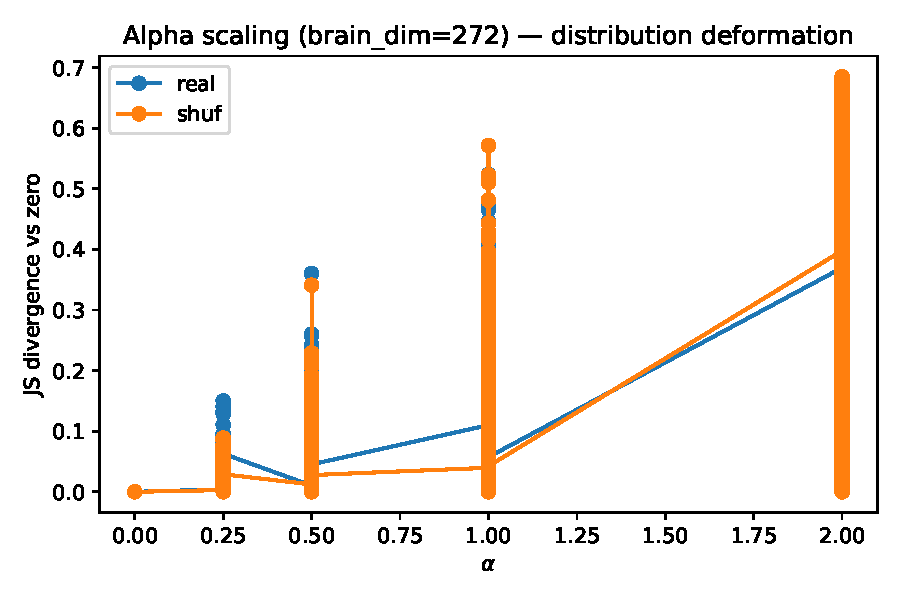
\includegraphics[width=0.48\linewidth]{figs/js_vs_alpha_272_clean.pdf}
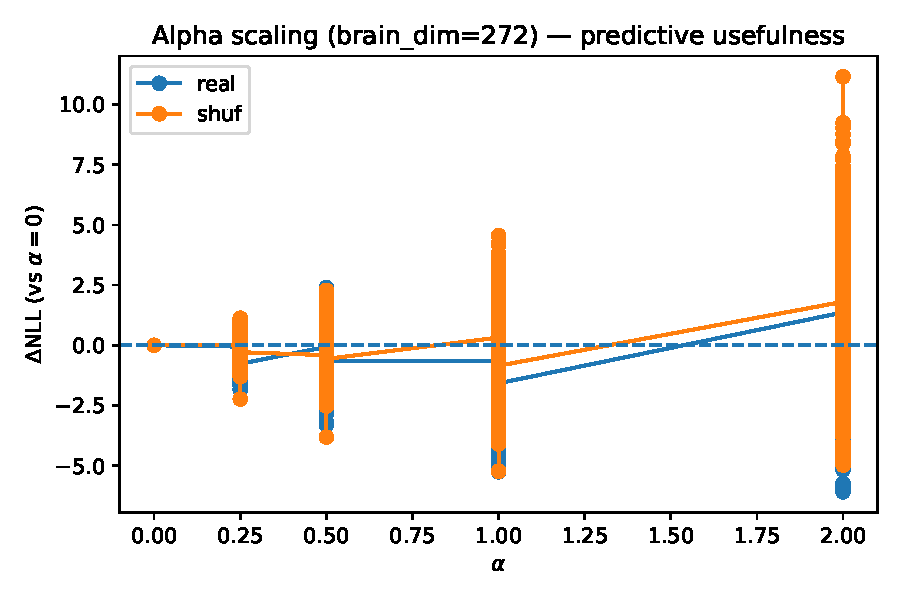
\includegraphics[width=0.48\linewidth]{figs/dnll_vs_alpha_272_clean.pdf}
\caption{Alpha scaling for the 272-D brain-conditioned LM. (Left) JS divergence vs.\ $\alpha$ relative to the $\alpha=0$ (zero-brain) baseline. (Right) $\Delta$NLL vs.\ $\alpha=0$. Real brain improves next-token prediction for moderate $\alpha$ (negative $\Delta$NLL), while shuffled brain degrades prediction despite comparable distributional deformation.}
\label{fig:alpha_scaling_272}
\end{figure}

\begin{figure}[h]
\centering
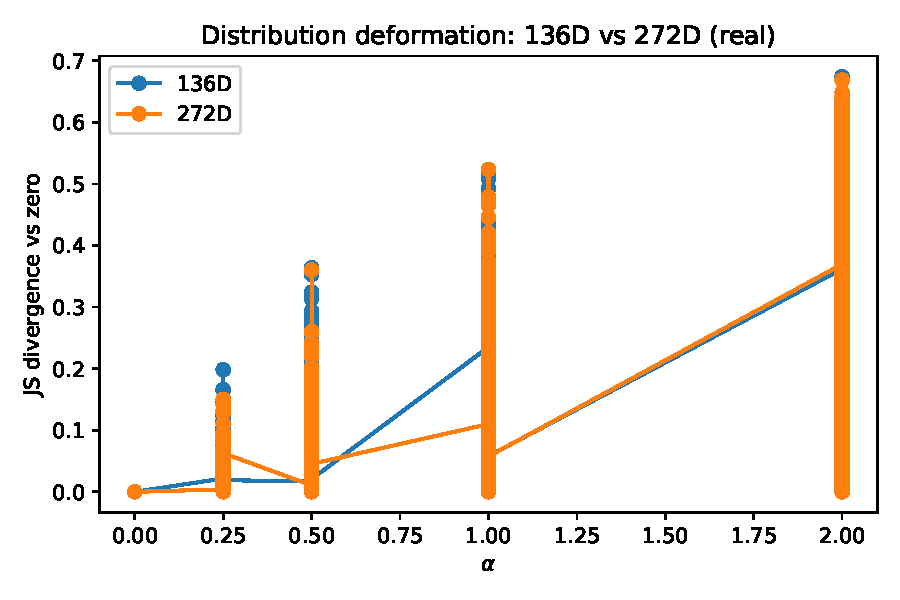
\includegraphics[width=0.48\linewidth]{figs/js_overlay_real_136_vs_272.pdf}
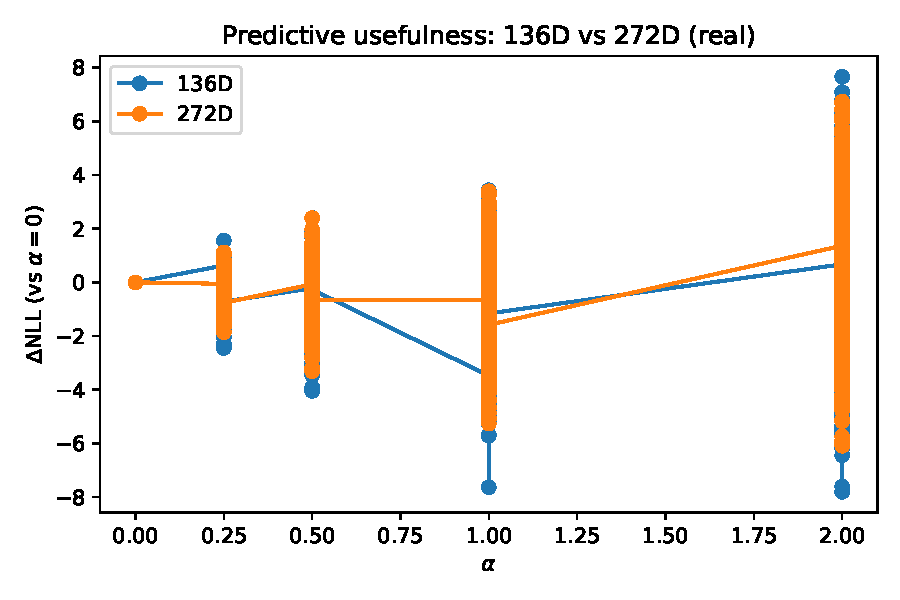
\includegraphics[width=0.48\linewidth]{figs/dnll_overlay_real_136_vs_272.pdf}
\caption{Direct comparison of alpha scaling between 136-D and 272-D models under the REAL condition. Overlaying curves on identical axes reveals differences in deformation strength (JS) and predictive usefulness ($\Delta$NLL) that can be visually subtle in separate plots.}
\label{fig:alpha_overlay_136_272}
\end{figure}

\begin{figure}[h]
\centering
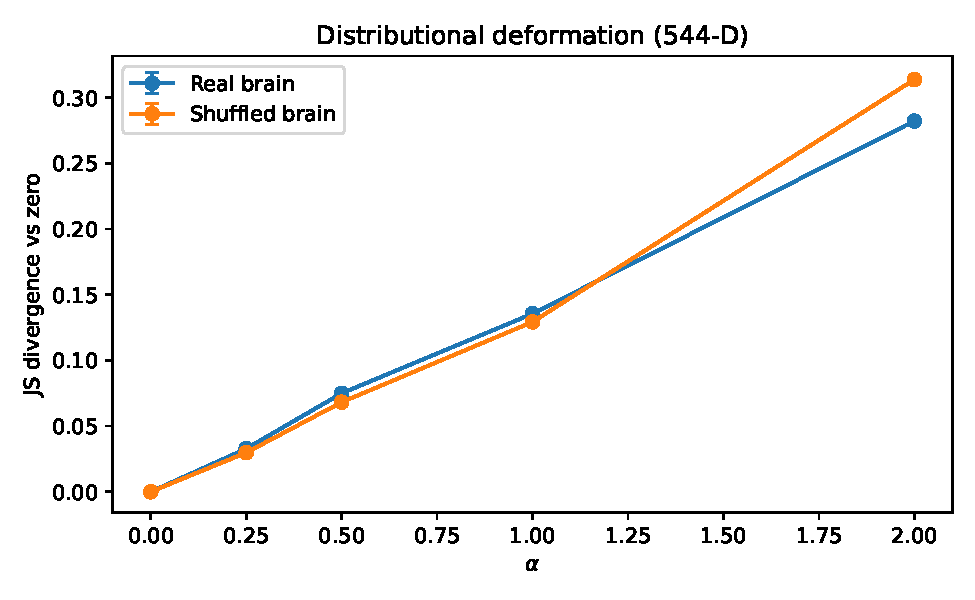
\includegraphics[width=0.48\linewidth]{figs/js_vs_alpha_544_clean.pdf}
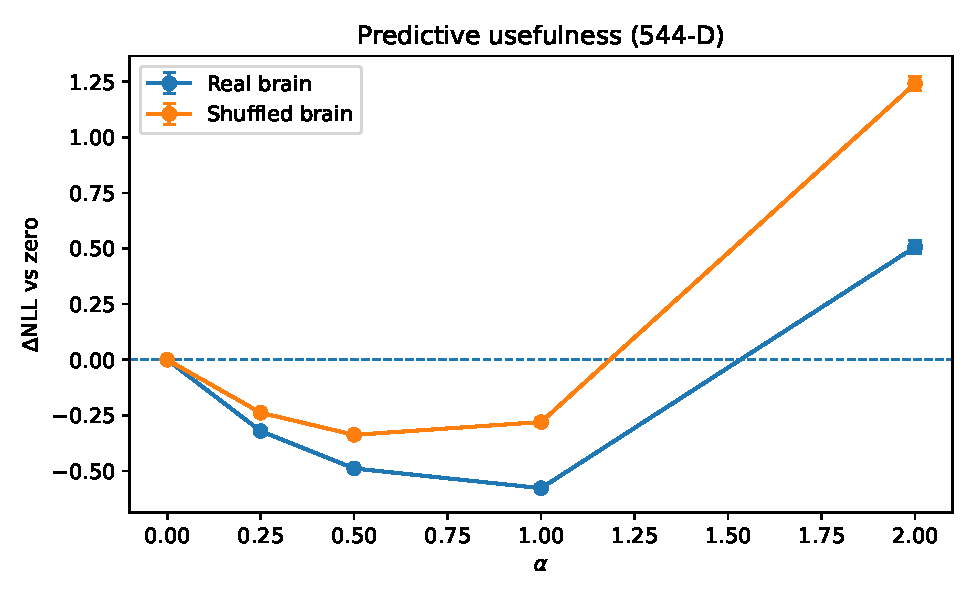
\includegraphics[width=0.48\linewidth]{figs/dnll_vs_alpha_544_clean.pdf}
\caption{Alpha scaling for the 544-D brain-conditioned LM. (Left) JS divergence vs.\ $\alpha$ relative to the $\alpha=0$ (zero-brain) baseline. (Right) $\Delta$NLL vs.\ $\alpha=0$. Both real and shuffled brain vectors induce smoothly increasing deformation, but real brain yields stronger predictive gains at moderate $\alpha$ and substantially less degradation at large $\alpha$.}
\label{fig:alpha_scaling_544}
\end{figure}

\section{Diagnostic Ablations for MEG-Conditioned T5}
\label{app:meg_t5_diagnostics}

This appendix reports additional MEG-MASC/T5 diagnostic runs used to interpret the real-neural pilot.
We include these results as ablations rather than as final benchmark claims.
All runs use target-only decoding, per-example brain normalization, and REAL/ZERO/SHUF evaluation.
Table~\ref{tab:meg_t5_appendix_controls} keeps the in-sample and peri-word diagnostics, Table~\ref{tab:meg_t5_appendix_heldout} summarizes the held-out post-word hybrid results reported in the main text, and Table~\ref{tab:meg_t5_appendix_windows} isolates early and late subwindows within the successful post-word window.
Table~\ref{tab:meg_t5_appendix_aux} then reports a matched-shape random auxiliary-stream baseline used to test whether any continuous side channel can reproduce the held-out MEG effect.

\begin{figure}[h]
\centering
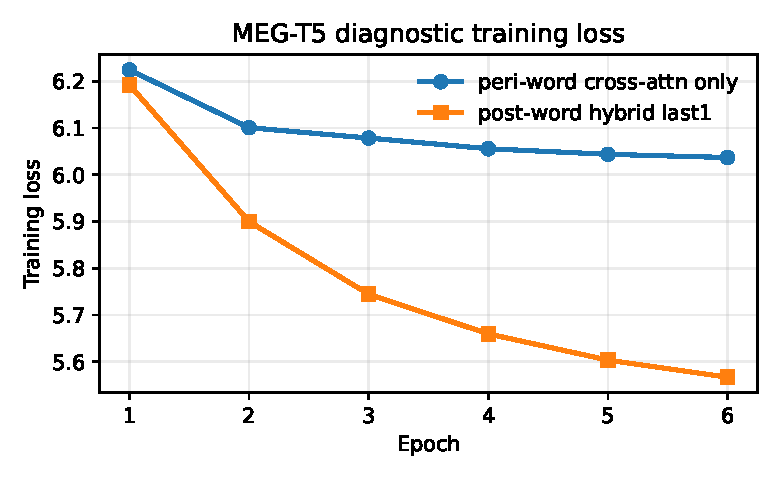
\includegraphics[width=0.65\linewidth]{figs/meg_t5_diagnostic_loss.pdf}
\caption{
Training loss for two overnight MEG-MASC/T5 diagnostic runs.
The post-word hybrid model reaches lower training loss than the peri-word cross-attention-only model, but training loss alone is not an alignment metric; the REAL/ZERO/SHUF controls in Table~\ref{tab:meg_t5_appendix_controls} determine whether the learned dependence is useful and pairing-specific.
}
\label{fig:meg_t5_diagnostic_loss}
\end{figure}

\begin{table*}[h]
\centering
\caption{
MEG-MASC/T5 diagnostic ablations.
Negative $\Delta$NLL means REAL is better than the control.
The cross-attention-only post-word row is the earlier conservative baseline.
The peri-word run shows that stronger use of brain input can be harmful relative to ZERO.
The hybrid row is a strong in-sample result; held-out validation is reported separately in Table~\ref{tab:meg_t5_appendix_heldout}.
}
\label{tab:meg_t5_appendix_controls}
\resizebox{\linewidth}{!}{%
\begin{tabular}{llcccccc}
\toprule
Setup & Window & Final train loss & NLL REAL & NLL ZERO & NLL SHUF & $\Delta$R-Z & $\Delta$R-S \\
\midrule
Post-word cross-attn only & $0.0$--$0.6$s & 6.0947 & 6.8936 & 6.9048 & 6.9011 & $-0.0112$ & $-0.0075$ \\
Peri-word cross-attn only & $-0.1$--$0.8$s & 6.0369 & 7.4154 & 7.1102 & 7.4818 & $+0.3052$ & $-0.0664$ \\
Post-word hybrid last1 & $0.0$--$0.6$s & 5.5670 & 5.9504 & 6.0718 & 6.0579 & $-0.1214$ & $-0.1074$ \\
\bottomrule
\end{tabular}
}
\end{table*}

\begin{table*}[h]
\centering
\caption{
Paired-control details for the MEG-MASC/T5 diagnostic ablations.
The hybrid model changes the predictive distribution much more strongly than the conservative cross-attention-only model, as reflected by lower top-1 agreement with ZERO.
}
\label{tab:meg_t5_appendix_paired}
\resizebox{\linewidth}{!}{%
\begin{tabular}{lcccccc}
\toprule
Setup & $\Delta$R-Z 95\% CI & $\Delta$R-S 95\% CI & Win R-Z & Win R-S & JS REAL & Top-1 R/Z \\
\midrule
Post-word cross-attn only & [$-0.0126$, $-0.0098$] & [$-0.0091$, $-0.0060$] & 0.5039 & 0.4937 & 0.0018 & 0.9997 \\
Peri-word cross-attn only & [$+0.2934$, $+0.3170$] & [$-0.0831$, $-0.0497$] & 0.4185 & 0.5001 & 0.0440 & 0.9517 \\
Post-word hybrid last1 & [$-0.1265$, $-0.1163$] & [$-0.1118$, $-0.1030$] & 0.5503 & 0.5588 & 0.0140 & 0.9146 \\
\bottomrule
\end{tabular}
}
\end{table*}

\begin{table*}[h]
\centering
\caption{
Held-out post-word hybrid results for MEG-MASC/T5.
Random held-out, story-blocked, and subject-blocked evaluation all preserve the REAL $<$ ZERO and REAL $<$ SHUF control pattern.
}
\label{tab:meg_t5_appendix_heldout}
\resizebox{\linewidth}{!}{%
\begin{tabular}{lcccccccc}
\toprule
Split & $n$ & $\Delta$R-Z 95\% CI & $\Delta$R-S 95\% CI & Win R-Z & Win R-S & JS REAL & JS SHUF & Top-1 R/Z \\
\midrule
Random held-out & 17{,}976 & [$-0.1141$, $-0.0974$] & [$-0.1232$, $-0.1079$] & 0.5309 & 0.5595 & 0.0157 & 0.0159 & 0.8745 \\
Story-blocked & 50{,}000 & [$-0.1092$, $-0.1004$] & [$-0.0818$, $-0.0738$] & 0.5491 & 0.5371 & 0.0088 & 0.0088 & 0.8997 \\
Subject-blocked & 34{,}240 & [$-0.0845$, $-0.0744$] & [$-0.0871$, $-0.0776$] & 0.5386 & 0.5465 & 0.0103 & 0.0104 & 0.9954 \\
\bottomrule
\end{tabular}
}
\end{table*}

\begin{table*}[h]
\centering
\caption{
Leave-one-subject-out (LOSO) summary for the post-word hybrid MEG-MASC/T5 model.
Each of the 11 subjects is held out once for testing.
All subject-level REAL-ZERO and REAL-SHUF 95\% confidence intervals remain below zero.
}
\label{tab:meg_t5_appendix_loso}
\resizebox{0.9\linewidth}{!}{%
\begin{tabular}{lccccc}
\toprule
Subjects & Total held-out $n$ & Mean $\Delta$R-Z & s.d. & Mean $\Delta$R-S & s.d. \\
\midrule
11 held-out subjects & 179{,}760 & $-0.0819$ & 0.0189 & $-0.0796$ & 0.0233 \\
\bottomrule
\end{tabular}
}
\end{table*}

\begin{table*}[h]
\centering
\caption{
Matched-shape auxiliary-stream null baseline on the story-blocked split.
Each MEG window is replaced with a Gaussian auxiliary stream of the same temporal shape, and the same T5 architecture is retrained from scratch.
The auxiliary stream does not produce a pairing-specific advantage: REAL and SHUF are indistinguishable and both remain near the ZERO baseline.
}
\label{tab:meg_t5_appendix_aux}
\resizebox{\linewidth}{!}{%
\begin{tabular}{lccccccccc}
\toprule
Auxiliary input & $n$ & NLL REAL & NLL ZERO & NLL SHUF & $\Delta$R-Z & 95\% CI & $\Delta$R-S & 95\% CI & Top-1 R/Z \\
\midrule
Gaussian iid stream & 50{,}000 & 7.2048 & 7.2057 & 7.2048 & $-0.0008$ & [$-0.0010$, $-0.0006$] & $+0.0000$ & [$-0.0002$, $+0.0002$] & 0.9994 \\
\bottomrule
\end{tabular}
}
\end{table*}

\begin{table*}[h]
\centering
\caption{
Story-blocked temporal ablation for the post-word hybrid MEG-MASC/T5 model.
The full $0.0$--$0.6$ s window is strongest; the early half is effectively null, the late half retains only a weaker effect, and a narrow late slice fails.
}
\label{tab:meg_t5_appendix_windows}
\resizebox{\linewidth}{!}{%
\begin{tabular}{lccccccc}
\toprule
Window & Brain len & NLL REAL & NLL ZERO & NLL SHUF & $\Delta$R-Z & $\Delta$R-S & Top-1 R/Z \\
\midrule
$0.0$--$0.6$s & 120 & 7.1885 & 7.2933 & 7.2663 & $-0.1048$ & $-0.0778$ & 0.8997 \\
$0.0$--$0.3$s & 60 & 7.5321 & 7.5322 & 7.5322 & $-0.0001$ & $-0.0000$ & 1.0000 \\
$0.3$--$0.6$s & 60 & 7.1834 & 7.2061 & 7.2040 & $-0.0227$ & $-0.0206$ & 0.9976 \\
$0.45$--$0.6$s & 30 & 7.1964 & 7.1959 & 7.1963 & $+0.0005$ & $+0.0001$ & 0.9999 \\
\bottomrule
\end{tabular}
}
\end{table*}

\subsection{Cross-Attention Timing in the Story-Blocked Model}
\label{app:meg_t5_attention}

To inspect where the successful story-blocked post-word model reads the MEG window, we export decoder cross-attention for the final prediction step over 5{,}000 held-out examples and average over decoder layers and heads.
Figure~\ref{fig:meg_t5_attention_story_real} shows a pronounced late-window preference.
The last quarter of the post-word window ($450$--$600$ ms after word onset) carries $50.9\%$ of the mean attention mass, compared with $15.5\%$, $13.4\%$, and $20.2\%$ for the first three quarters.
The mean peak occurs at bin $107$ out of $120$, corresponding to approximately $535$ ms after word onset, and the 10th, median, and 90th percentiles of the peak bin are all $107$.
This suggests that the model relies primarily on late post-word neural activity, but the near-fixed peak location also indicates a strong positional bias rather than highly example-specific temporal routing.

We then compare this timing profile against a shuffled-brain control using the same story-blocked examples.
The resulting attention curves are nearly indistinguishable (Figure~\ref{fig:meg_t5_attention_story_compare}).
REAL assigns $50.87\%$ of its mass to the final quarter of the window, versus $50.82\%$ for SHUF; the mean peak time differs by only $0.015$ ms ($535.096$ vs.\ $535.111$ ms); and normalized attention entropy is almost identical ($0.9508$ vs.\ $0.9509$).
Thus, while the successful model clearly prefers late post-word activity, the temporal \emph{location} of attention does not by itself separate matched from mismatched MEG.
The pairing-specific signal appears in the NLL controls, not in a more selective attention-timing profile.

\begin{figure*}[t]
\centering
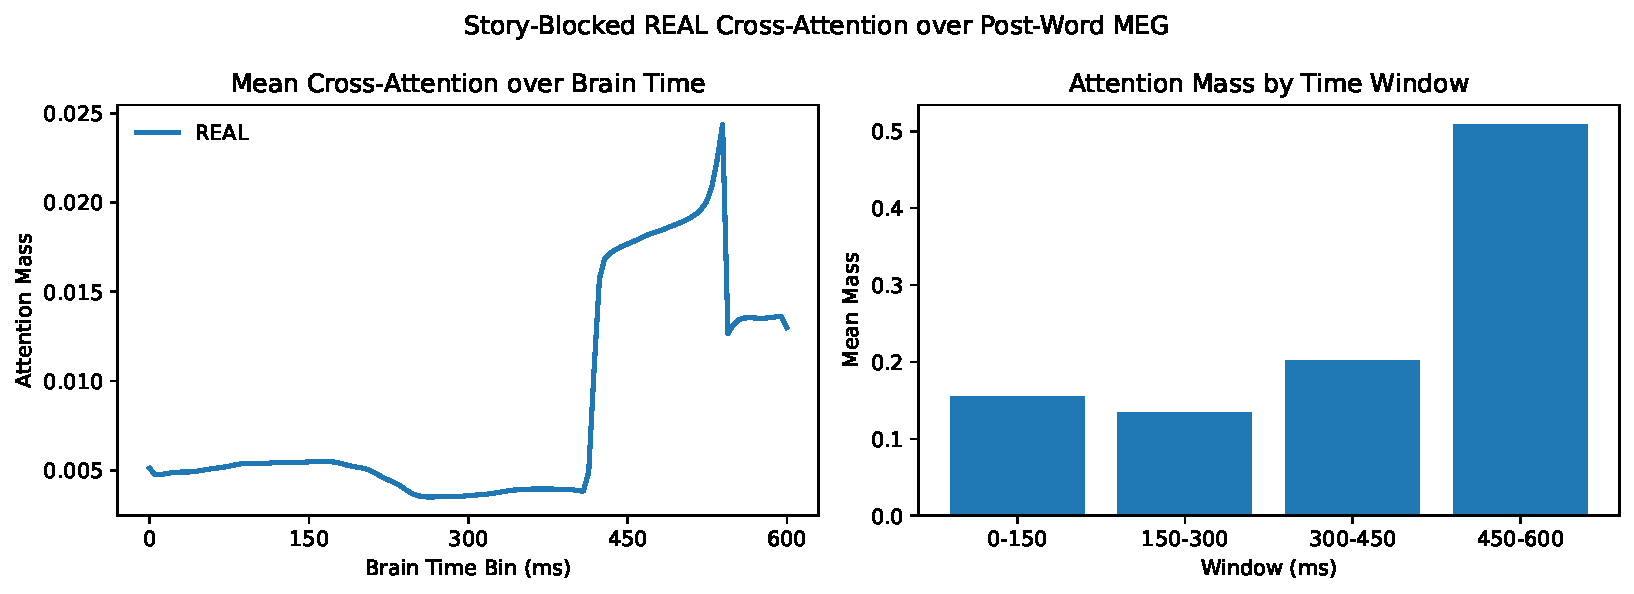
\includegraphics[width=0.9\linewidth]{figs/meg_t5_attention_story_real.pdf}
\caption{
Mean decoder cross-attention over the post-word MEG window for the story-blocked post-word hybrid model, averaged across 5{,}000 held-out examples.
Left: mean attention curve for the final decoder prediction step.
Right: attention mass aggregated over four equal-width time windows.
The model concentrates roughly half of its attention mass in the final quarter of the $0.0$--$0.6$ s post-word window, with a consistent peak around $535$ ms after onset.
}
\label{fig:meg_t5_attention_story_real}
\end{figure*}

\begin{figure*}[t]
\centering
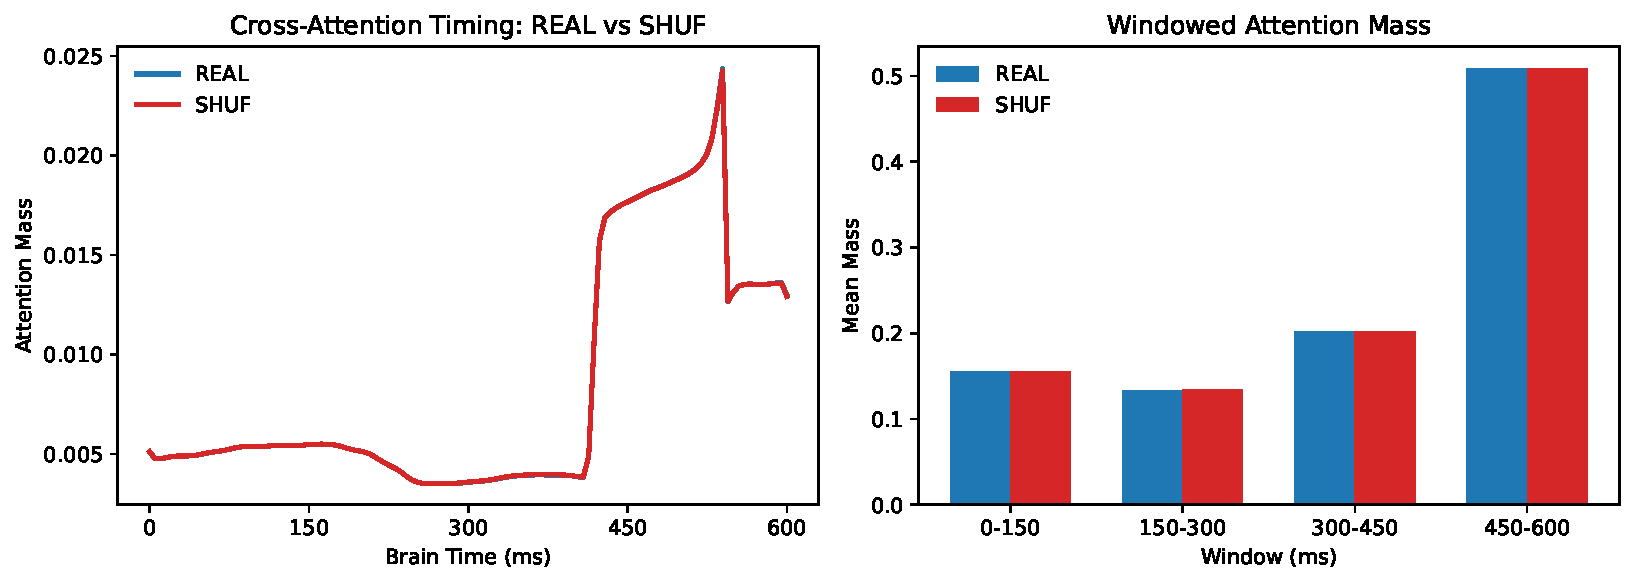
\includegraphics[width=0.9\linewidth]{figs/meg_t5_attention_story_real_vs_shuf.pdf}
\caption{
Comparison of decoder cross-attention timing for REAL and SHUF MEG on the same 5{,}000 story-blocked examples.
The two curves are nearly identical: both peak at approximately $535$ ms after onset and allocate about half of their total attention mass to the final quarter of the post-word window.
This indicates that the successful model's attention timing is dominated by a late-window positional preference rather than a visibly sharper or differently located REAL-specific temporal focus.
}
\label{fig:meg_t5_attention_story_compare}
\end{figure*}

These ablations support three practical conclusions.
First, loss curves are necessary but insufficient: the peri-word run optimizes, yet REAL is substantially worse than ZERO.
Second, temporal structure matters within the successful post-word window itself: the early half is effectively null, the late half is only weakly useful, and the narrow late slice fails, so the main effect is distributed across the broader $0.0$--$0.6$ s response rather than reducible to a single late peak.
Third, increasing trainable capacity by unfreezing the last T5 block can dramatically improve controls, and the new held-out tables show that this gain is not purely in-sample.
Random held-out, story-blocked, subject-blocked, and LOSO evaluation all preserve a clear REAL advantage over ZERO and SHUF, while the peri-word variant remains a cautionary example that stronger brain dependence can still be harmful.



%%%%%%%%%%%%%%%%%%%%%%%%%%%%%%%%%%%%%%%%%%%%%%%%%%%%%%%%%%%%%%%%%%%%%%%%%%%%%%%
%%%%%%%%%%%%%%%%%%%%%%%%%%%%%%%%%%%%%%%%%%%%%%%%%%%%%%%%%%%%%%%%%%%%%%%%%%%%%%%


\newpage
\input{checklist.tex}

\end{document}
